% ----------------------------------------------------------------------
%  Set the document class
% ----------------------------------------------------------------------
\documentclass[11pt,a4paper]{article}
\usepackage[lmargin=2cm, tmargin=3cm, rmargin=2cm, bmargin=2cm, headheight=5cm]{geometry}

% ----------------------------------------------------------------------
% Define external packages, language, margins, fonts and new commands
% ----------------------------------------------------------------------
%\input{preamble} 
\usepackage[utf8]{inputenc}   % <<<<< Linux
\usepackage[english]{babel} % <<<<< English
\usepackage{notoccite}
\usepackage[skip=0.5\baselineskip]{caption}
\hyphenation{GTKWave}
\usepackage{listings}
\usepackage[all]{nowidow}
\usepackage{graphicx}
\usepackage[numbers,sort&compress]{natbib} % <<<<< References in numbered list [1],[2],...
\usepackage{subcaption} 
\usepackage{mdframed}
\usepackage{fancyhdr}
\usepackage{float}
\usepackage{mathtools}
\usepackage{hyperref}
\usepackage{comment}
\hypersetup{
    colorlinks,
    citecolor=black,
    filecolor=black,
    linkcolor=black,
    urlcolor=black
}

%\usepackage{setspace}
\renewcommand{\baselinestretch}{1.5}

%Header
\pagestyle{fancy}{
\fancyhf{}
\rhead{\includegraphics[width=30mm]{../../figlib/IST_A_CMYK_POS.pdf}}
\lhead{Grupo 67}

%footer
\lfoot{Lisbon, April 5, 2021}
\rfoot{Page \thepage}
}


%%%%%%%%%%%%%%%%%%%%%%%%%%%%%%%%%%%%%%%%%%%%%%%%%%%%%%%%%%%%%%%%%%%%%%%%
%     Begin Document                                                   %
%%%%%%%%%%%%%%%%%%%%%%%%%%%%%%%%%%%%%%%%%%%%%%%%%%%%%%%%%%%%%%%%%%%%%%%%

\begin{document}



% Set roman numbering (i,ii,...) before the start of chapters
%\pagenumbering{roman}

% ----------------------------------------------------------------------
%  Cover page
% ----------------------------------------------------------------------
\thispagestyle {empty}{

% IST Logo - Signature A
% parameters: bb=llx lly urx ury (bounding box), width=h_length, height=v_length, angle=angle, scale=factor, clip=true/false, draft=true/false. 
\includegraphics[bb=9.5cm 11cm 0cm 0cm,scale=0.29]{../../figlib/IST_A_CMYK_POS.pdf}

\begin{center}
%
% Figure (Image or plot)
%\vspace{1.0cm}
% height = 50 mm
%\includegraphics[height=50mm]{Figures/Airbus_A350.jpg}

% Title, author and degree
\textsc{\Large{ RC Circuit Analysis}}\\[0.5cm] % <<<<< EDIT TITLE
\vspace{0.6cm}
\textsc{\Large Circuit Theory and Electronics Fundamentals}\\[0.5cm]% <<<<< EDIT COURSE
\vspace{0.6cm}
\textsc{\large Filipe Valquaresma, 96375}\\[0.1cm]% <<<<< EDIT COURSE
\vspace{0.05cm}
\textsc{\large João Gaspar, 96406}\\[0.1cm]% <<<<< EDIT COURSE
\vspace{0.05cm}
\textsc{\large Leonardo Eitner, 96420}\\[0.1cm]% <<<<< EDIT COURSE
\vspace{0.6cm}
\textsc{\large Laboratory T2}\\[0.2cm]
\vspace{0.6cm}% <<<<< EDIT Report
\textsc{\large April 5, 2021}\\[0.2cm]
\vspace{0.6cm}% <<<<< EDIT DATE (corresponds to date of oral examination)


\end{center}
}

\pagestyle{fancy}


% ----------------------------------------------------------------------
% Dedication page (optional)
% ----------------------------------------------------------------------
%\input{dedication} 
%\cleardoublepage

% ----------------------------------------------------------------------
%  Acknowledgments (optional)
% ----------------------------------------------------------------------
%\input{acknowledgements}
%\cleardoublepage

% ----------------------------------------------------------------------
%  Abstract (both in English and Portuguese)
% ----------------------------------------------------------------------
%\input{resumo} 
%\cleardoublepage

%\input{abstract} 

% ----------------------------------------------------------------------
%  Table of contents, list of tables, list of figures and nomenclature
% ----------------------------------------------------------------------

% Table of contents

\tableofcontents

% List of tables
%\addcontentsline{toc}{section}{\listtablename}
%\listoftables
%\cleardoublepage 

% List of figures
%\addcontentsline{toc}{section}{\listfigurename}
%\listoffigures
%\cleardoublepage 

% Set arabic numbering (1,2,...) after preface
%
%\setcounter{page}{1}
%\pagenumbering{arabic}

% ----------------------------------------------------------------------
%  Body
% ----------------------------------------------------------------------

\pagebreak
\setcounter{page}{1}
\section{Introduction}
\label{sec:introduction}

% state the learning objective 

\indent

The objective of this laboratory assignment is to create a circuit that works as an {\bf audio amplifier}. 

An audio amplifier is a device that aims to amplify the intensity of a sound, given as an input, while avoiding the introduction of noise or sound deformation. 

This circuit does not process sound waves. It receives as an input an analog electrical signal, which is a processed sound wave (for example, by a microphone), and amplifies it, producing an amplified analog electrical signal as an output. 

The main challenge is to find a good balance between cost of production, width of the pass-band, and gain, i.e. a non-expensive amplifier that is able to increase the sound amplitude without significant losses in higher and lower frequencies. 

The circuit, which can be seen on the following figure (Figure \ref{fig:schematic}), is composed by two stages: the \textit{gain stage} and the \textit{output stage}. 
These two stages work in complement to each other: the \textit{gain stage}, which aims to increase the magnitude of the signal, without much concern for the output impedance, while the \textit{output stage}, aims to convert the output impedance into something acceptable for the desired load (in this case it is $8 k\Omega$), without affecting the previous gain.


\begin{figure}[h!]
    \centering
    \includegraphics[width = 0.8\linewidth]{fig0.pdf}
    \caption{Audio amplifier circuit}
    \label{fig:schematic}
\end{figure}

In Section~\ref{sec:analysis}, a theoretical analysis of the circuit is
presented. In Section~\ref{sec:simulation}, the circuit is analysed by
simulation, and the results are compared to the theoretical results obtained in Section~\ref{sec:analysis}. The conclusions of this study are outlined in Section~\ref{sec:conclusion}.


\pagebreak
\section{Theoretical Analysis}
\label{sec:analysis}
\indent

In this section, the circuit shown in Figure~\ref{fig:rc} is analysed
theoretically, using the mesh and the node methods. 

\subsection{Mesh analysis}
%imagem
\begin{figure}[H] \centering
    \includegraphics[width=0.8\linewidth]{Images/mesh analysis.pdf}
    \caption{Current flow by mesh.}
    \label{fig:Currents}
\end{figure}


\indent

This circuit is composed by four primary meshes in which we assume the current flows counter-clockwise in every mesh but one, as seen in Figure~\ref{fig:Currents}.

Note that this is merely a convention used in our theoretical computations. The actual physical direction of the current can be obtained by analysing the algebraic sign of the current in each branch. 

To find out the current that flows in each mesh we use the Kirchhoff Voltage Law (KVL) followed by Ohm's Law. 

\begin{equation}
    \sum_{k=1}^{n} V_k = 0.
    \quad\text{,}\quad 
    V=RI.
\end{equation}

In some cases, two currents flow on the same branch. To solve this we use  Kirchhoff Current Law (KCL), to find the current on that branch.

\begin{equation}
    \sum_{k=1}^{n} I_k = 0.
    \label{eq:KCL}
\end{equation}

In mesh $a$ (mesh where the current $I_a$ flows) we assume that the voltage source is providing energy to the circuit and therefore the current has to flow clock-wise. This means that the sum of the voltages in each resistor ($R_1$, $R_3$ and $R_4$) has to equal the voltage $V_a$.

In meshes $b$, $c$ and $d$ we followed the same process as in mesh $a$, defining the way in which the current flows through current and voltage sources.
To exemplify this process, the equation for mesh $a$ is the following:

\begin{equation}
    V_a=R_1I_a+R_3(I_a+I_b)+R_4(I_a+I_c).
\end{equation}

With the aid of octave, we can solve the four equations to obtain the following table (table~\ref{tab:Imesh}).

\begin{table}[h]
  \centering
  \begin{tabular}{|l|r|}
    \hline    
    {\bf Name} & {\bf Value [mA]} \\ \hline
    Ia & 0.173163 \\ \hline 
Ib & 0.001232 \\ \hline 
Ic & 0.856152 \\ \hline 
Id & 1.034000 \\ \hline 

  \end{tabular}
  \caption{Results from the mesh analysis, from \textit{Octave}.}
  \label{tab:Imesh}
\end{table}

Since we know the current on each mesh we can calculate the current on every branch. The results are present on table~\ref{tab:Ibranch}.

\begin{table}[h]
  \centering
  \begin{tabular}{|l|r|}
    \hline    
    {\bf Name} & {\bf Value [mA]} \\ \hline
    Ib & -0.204136 \\ \hline 
Id & 0.000000 \\ \hline 
R1 & 0.194523 \\ \hline 
R2 & -0.204136 \\ \hline 
R3 & -0.009614 \\ \hline 
R4 & 1.156284 \\ \hline 
R5 & 0.204136 \\ \hline 
R6 & 0.961761 \\ \hline 
R7 & 0.961761 \\ \hline 

  \end{tabular}
  \caption{Current on each branch.}
  \label{tab:Ibranch}
\end{table}


\subsection{Node analysis}

\begin{figure}[H] \centering
    \includegraphics[width=0.8\linewidth]{Images/node analysis.pdf}
    \caption{Nodes.}
    \label{fig:Nodes}
\end{figure}

\indent

There are 8 nodes in total which means that we need 8 equations to find out the voltages in each node and solve the circuit. Therefore, we use the Kirchhoff Current Law (KCL, equation~\ref{eq:KCL}) in every node that is not connected to a voltage source (nodes 2, 3, 6 and 7, which are identified in Figure~\ref{fig:Nodes} ).

We assume node 4 ($V_4$) as the reference node, which means that its value is 0. This node was chosen because usually, the negative terminal of a voltage source is connected to the ground.

It is also known that the value of a voltage source is equivalent to the difference of the voltages in each node to which the source is connected. That allows us to create two more equations, since there are two voltage sources in the circuit.

For the $8^{th}$ equation we can create a supernode with nodes 5 and 8 since the dependent voltage source is not connected to the reference node. This way, nodes 5 and 8 are considered as one by ignoring the voltage source between them.

To demonstrate the process, the node 2 equation resulting from the KCL application is the following:

\begin{equation}
    (V_2-V_3)G_2=(V_5-V_2)G_3+(V_1-V_2)G_1.
\end{equation}

Doing this on all possible nodes/supernode and adding the extra equations, regarding the voltage sources, a system of linear equations can be obtained and solved with the aid of \textit{Octave}. The results are presented on table~\ref{tab:Volts}.

\begin{table}[h]
  \centering
  \begin{tabular}{|l|r|}
    \hline    
    {\bf Name} & {\bf Value [V]} \\ \hline
    V1 & 5.008942 \\ \hline 
V2 & 4.808960 \\ \hline 
V3 & 4.394160 \\ \hline 
V4 & -0.000000 \\ \hline 
V5 & 4.837861 \\ \hline 
V6 & 5.474754 \\ \hline 
V7 & -2.008722 \\ \hline 
V8 & -2.970916 \\ \hline 

  \end{tabular}
  \caption{Results from the node analysis, from \textit{Octave}.}
  \label{tab:Volts}
\end{table}


\pagebreak
\section{Simulation Analysis}
\label{sec:simulation}


%Introduzir a cena do ngspice costume
%Mostrar a cena optimizada e explicar o porque de termos usado estes valores diferentes

\indent
 
 This section discusses the circuit simulation, performed using {\it Ngspice}. 

This circuit was entered into the {\it Ngspice} simulation environment. This tool is used to simulate analog electronic circuits and predict circuit behaviour. 

After having the base circuit description, the parameters have been chosen by trial and error. The final values are present on the following table (table \ref{tab:InputParam}):

\begin{table}[H]
  \centering
  \begin{tabular}{|l|r|}
    \hline    
    {\bf Name} & {\bf Value} \\ \hline
    \input{../Analysis/inputs.tex}
  \end{tabular}
  \caption{Input Parameters}
  \label{tab:InputParam}
\end{table}


In this iterative progress, we arrived at these conclusions about each main parameter:
 
\begin{itemize}
    \item\textbf{Effect of the Coupling Capacitors:}
    The coupling capacitor's main purpose is to neglect any constant current values in order to ensure that the transistors are always in F.A.R.. A consequence that may come from this is the blocking of some low frequencies, lowering therefore the bandwidth.

    \item\textbf{Effect of the Bypass Capacitor:}
    The bypass capacitor $C_b$ is used in order to neutralize the negative impact that the resistor $R_e$ has on the gain. By putting both components in parallel, the capacitor works as a bypass neglecting the effect that the resistor has on the gain when the current is AC.  Meanwhile, when the current is DC, it acts as an open-circuit, allowing the resistor to do its job.
 
    \item\textbf{Effect of the Resistor $R_C$:}
    The resistor $R_C$ has a direct influence in the current $I_C$ which in turn determines the value of $g_m$. This value directly influences the gain. In summary the gain increases when $R_C$ increases and vice-versa.
\end{itemize}    

 


\subsection{Results}

\indent

With the parameters honed in, the OP analysis was possibly, visible on table \ref{tab:OP_ngs}:

\begin{table}[H]
  \centering
  \begin{tabular}{|l|r|}
    \hline    
    {\bf Name} & {\bf Value} \\ \hline
    @gcs[i] & 1.837491e-04\\ \hline
@id[current] & 1.033653e-03\\ \hline
@r1[i] & 1.924024e-04\\ \hline
@r2[i] & 1.837491e-04\\ \hline
@r3[i] & 8.653299e-06\\ \hline
@r4[i] & -1.14368e-03\\ \hline
@r5[i] & 8.499042e-04\\ \hline
@r6[i] & 9.512771e-04\\ \hline
@r7[i] & 9.512771e-04\\ \hline
v(1) & 5.008942e+00\\ \hline
v(2) & 4.811140e+00\\ \hline
v(3) & 4.437766e+00\\ \hline
v(4) & 0.000000e+00\\ \hline
v(5) & 4.785125e+00\\ \hline
v(6) & 2.133477e+00\\ \hline
v(7) & -1.98683e+00\\ \hline
v(8) & -2.93853e+00\\ \hline

  \end{tabular}
  \caption{OP Analysis}
  \label{tab:OP_ngs}
\end{table}

With a few calculations, it is possible to obtain the different values for the voltage across the terminals of both transistors:

\begin{table}[H]
  \centering
  \begin{tabular}{|l|r|}
    \hline    
    {\bf Name} & {\bf Value} \\ \hline
    @gcs[i] & -2.04136e-04\\ \hline
@r1[i] & 1.945228e-04\\ \hline
@r2[i] & -2.04136e-04\\ \hline
@r3[i] & -9.61339e-06\\ \hline
@r4[i] & 1.156284e-03\\ \hline
@r5[i] & 2.041377e-04\\ \hline
@r6[i] & 9.617611e-04\\ \hline
@r7[i] & 9.617611e-04\\ \hline
v(1) & 5.008942e+00\\ \hline
v(2) & 4.808960e+00\\ \hline
v(3) & 4.394160e+00\\ \hline
v(4) & 0.000000e+00\\ \hline
v(5) & 4.837861e+00\\ \hline
v(6) & 5.474758e+00\\ \hline
v(7) & -2.00872e+00\\ \hline
v(8) & -2.97092e+00\\ \hline

  \end{tabular}
  \caption{OP analysis deep dive}
  \label{tab:OP2_ngs}
\end{table}

As it can be seen, the differences are positive, which means that the voltage across the terminals is greater than the saturation voltage of the transistors, which in turn ensures that they are on the F.A.R..

After the OP analysis, it is possible to perform a frequency analysis, that can be seen on the next 2 graphs (Figure \ref{fig:FreqANGS}):

\begin{figure}[H]
\centering
\begin{subfigure}{.5\textwidth}
  \centering
  \includegraphics[width=.8\linewidth, trim={2cm 1.5cm 0.5cm 6cm}, clip]{../Simulation/vo2f_m.pdf}
  \caption{Magnitude}
\end{subfigure}%
\begin{subfigure}{.5\textwidth}
  \centering
  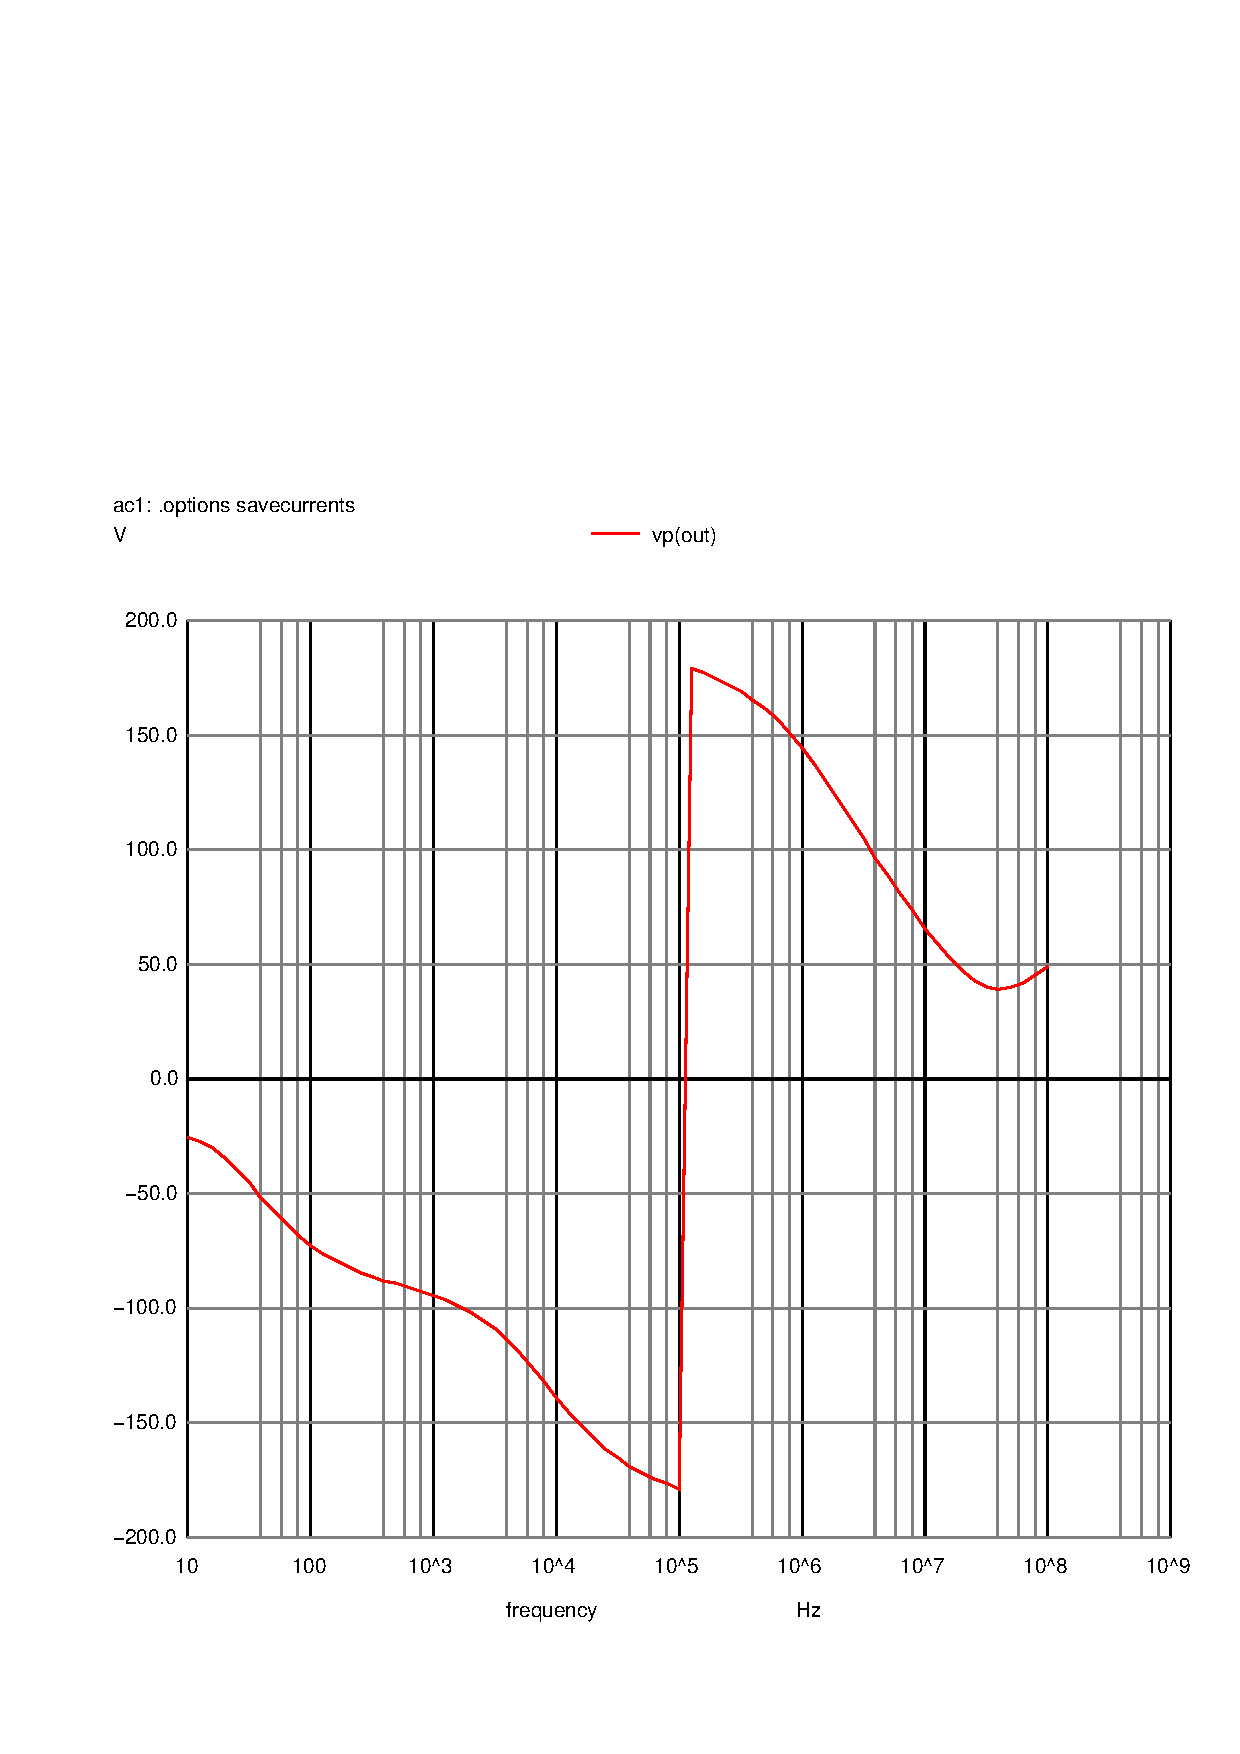
\includegraphics[width=.8\linewidth, trim={2cm 1.5cm 0.5cm 6cm}, clip]{../Simulation/vo2f_ph.pdf}
  \caption{Phase}
\end{subfigure}
\caption{Frequency analysis}
\label{fig:FreqANGS}
\end{figure}


With this done, the final parameter for the Audio amplifier can be obtained:

\begin{table}[H]
  \centering
  \begin{tabular}{|l|r|}
    \hline    
    {\bf Name} & {\bf Value} \\ \hline
    \input{../Simulation/freq_tab.tex}
  \end{tabular}
  \caption{Output parameters}
  \label{tab: OutputParamNGS}
\end{table}

As we can see, the impedances match what we expectected: the output impedance is low and similar to the resistance of the load, wheras the input impedance is high, which is desirable.


Finally, since there is no visible distortion on the next graph, it is possible to ensure that the signal is correctly amplified.


\begin{figure}[h!]
    \centering
  \includegraphics[width=.6\linewidth, trim={2cm 1.5cm 0.5cm 6cm}, clip]{../Simulation/vout.pdf}
  \caption{Transient analysis - Voltage output}
  \label{tab:TransNGS}
\end{figure}


As shown, the signal is greatly amplified and shows no visible distortions. One possible downside of this approach is that the phase of the output is not the same as the phase of the input. However, this is not a problem since the human ear is not sensible enough to notice it.


\pagebreak
\section{Result Analysis}
\label{sec:ResultAnalysis}

\indent

In this section the results will firstly be analysed and then compared, identifying the differences between the calculated results and the simulation results. The relative differences are calculated according to equation \ref{eq:error}:

\begin{equation}
    e_r = \frac{V_{Octave}-V_{ngspice}}{V_{Octave}} \hspace{5pt}
    \label{eq:error}
\end{equation}

\subsection{Circuit analysis for $t<0$}


\begin{table}[H]
    \caption{Results from the first analysis}
    \begin{subtable}{.5\linewidth}
      \centering
        \caption{Octave}
        \begin{tabular}{ll}
        \hline    
        {\bf Name} & {\bf Value [V]} \\ \hline
        V1 & 5.008942 \\ \hline 
V2 & 4.808960 \\ \hline 
V3 & 4.394160 \\ \hline 
V4 & -0.000000 \\ \hline 
V5 & 4.837861 \\ \hline 
V6 & 5.474754 \\ \hline 
V7 & -2.008722 \\ \hline 
V8 & -2.970916 \\ \hline 

        \end{tabular}
        \begin{tabular}{ll}
        \hline    
        {\bf Name} & {\bf Value [A]} \\ \hline
        Ib & -0.204136 \\ \hline 
Id & 0.000000 \\ \hline 
R1 & 0.194523 \\ \hline 
R2 & -0.204136 \\ \hline 
R3 & -0.009614 \\ \hline 
R4 & 1.156284 \\ \hline 
R5 & 0.204136 \\ \hline 
R6 & 0.961761 \\ \hline 
R7 & 0.961761 \\ \hline 

        \end{tabular}
        \label{tab:OpVOc}
    \end{subtable}%
    \begin{subtable}{.5\linewidth}
      \centering
        \caption{Ngspice}
        \begin{tabular}{ll}
        \hline    
        {\bf Name} & {\bf Value [A or V]} \\ \hline
        @gcs[i] & 1.837491e-04\\ \hline
@id[current] & 1.033653e-03\\ \hline
@r1[i] & 1.924024e-04\\ \hline
@r2[i] & 1.837491e-04\\ \hline
@r3[i] & 8.653299e-06\\ \hline
@r4[i] & -1.14368e-03\\ \hline
@r5[i] & 8.499042e-04\\ \hline
@r6[i] & 9.512771e-04\\ \hline
@r7[i] & 9.512771e-04\\ \hline
v(1) & 5.008942e+00\\ \hline
v(2) & 4.811140e+00\\ \hline
v(3) & 4.437766e+00\\ \hline
v(4) & 0.000000e+00\\ \hline
v(5) & 4.785125e+00\\ \hline
v(6) & 2.133477e+00\\ \hline
v(7) & -1.98683e+00\\ \hline
v(8) & -2.93853e+00\\ \hline

        \end{tabular}
        \label{tab:OpNgs}
    \end{subtable} 
    \label{tab:Op}
\end{table}

The values match almost perfectly. On the table below, the differences are studied with more detail.

\begin{table}[H]
    \caption{Differences on the first analysis}
    \begin{subtable}{.5\linewidth}
      \centering
        \caption{Voltages}
        \begin{tabular}{ll}
        \hline    
        {\bf Name} & {\bf Value [V]} \\ \hline
        \input{../Comparison/Voltages_diff.tex}
        \end{tabular}
        \label{tab:OpVDiff}
    \end{subtable}%
    \begin{subtable}{.5\linewidth}
      \centering
        \caption{Currents}
        \begin{tabular}{ll}
        \hline    
        {\bf Name} & {\bf Value [A]} \\ \hline
        \input{../Comparison/Currents_diff.tex}
        \end{tabular}
        \label{tab:OpCDiff}
    \end{subtable} 
    \label{tab:OpDiff}
\end{table}

This results are commented and explained on the next subsection (subsection \ref{subsection:CAVS}) since they require the same explanation.

\subsection{Circuit analysis for a voltage source-equivalent capacitor}
\label{subsection:CAVS}
\begin{table}[H]
    \caption{Results from the second analysis}
    \begin{subtable}{.5\linewidth}
      \centering
        \caption{Octave}
        \begin{tabular}{ll}
        \hline    
        {\bf Name} & {\bf Value [V]} \\ \hline
        \input{../Analysis/Voltages_2.tex}
        \end{tabular}
        \begin{tabular}{ll}
        \hline    
        {\bf Name} & {\bf Value [A]} \\ \hline
        \input{../Analysis/BranchCurrents_2.tex}
        \end{tabular}
        \label{tab:Op2Oc}
    \end{subtable}%
    \begin{subtable}{.5\linewidth}
      \centering
        \caption{Ngspice}
        \begin{tabular}{ll}
        \hline    
        {\bf Name} & {\bf Value [A or V]} \\ \hline
        @gcs[i] & -2.04136e-04\\ \hline
@r1[i] & 1.945228e-04\\ \hline
@r2[i] & -2.04136e-04\\ \hline
@r3[i] & -9.61339e-06\\ \hline
@r4[i] & 1.156284e-03\\ \hline
@r5[i] & 2.041377e-04\\ \hline
@r6[i] & 9.617611e-04\\ \hline
@r7[i] & 9.617611e-04\\ \hline
v(1) & 5.008942e+00\\ \hline
v(2) & 4.808960e+00\\ \hline
v(3) & 4.394160e+00\\ \hline
v(4) & 0.000000e+00\\ \hline
v(5) & 4.837861e+00\\ \hline
v(6) & 5.474758e+00\\ \hline
v(7) & -2.00872e+00\\ \hline
v(8) & -2.97092e+00\\ \hline

        \end{tabular}
        \label{tab:Op2Ngs}
    \end{subtable} 
    \label{tab:Op2}
\end{table}


\indent

An interesting result appears from this procedure: we notice that the current flows exclusively on the capacitor's mesh (mesh D), on resistor R5. This is explained by the fact that \emph{"current always flows through the path of least resistance"}: since the linearly dependent voltage source has voltage 0 in this instant, it is equivalent to a conductor wire with 0 resistance, configuring a closed circuit with only one resistor (R5). This result appears on table \ref{tab:Op2}.

\begin{table}[H]
    \caption{Differences on the second analysis}
    \begin{subtable}{.5\linewidth}
      \centering
        \caption{Voltages}
        \begin{tabular}{ll}
        \hline    
        {\bf Name} & {\bf Value [V]} \\ \hline
        \input{../Comparison/Voltages_2_diff.tex}
        \end{tabular}
        \label{tab:Op_2VDiff}
    \end{subtable}%
    \begin{subtable}{.5\linewidth}
      \centering
        \caption{Currents}
        \begin{tabular}{ll}
        \hline    
        {\bf Name} & {\bf Value [A]} \\ \hline
        \input{../Comparison/Currents_2_diff.tex}
        \end{tabular}
        \label{tab:Op_2CDiff}
    \end{subtable} 
    \label{tab:Op_2Diff}
\end{table}


The simulation results from both these procedures (table \ref{tab:OpDiff} and \ref{tab:Op_2Diff}) match the predicted ones from the theoretical analysis with great precision (errors are mostly in the range of $10^{-4}\%$). This was expected due to the fact that this circuit only contains linear (dependent and independent) components. The capacitor was not included since it was replaced by a simplified version (an open circuit or a voltage source, respectively).
One detail which is present on both tables is that "\textbf{NaN}" appears on some of the entries. This results from dividing 0 by 0 which happens when the predicted result by \textit{Octave} is 0 and the difference between \textit{Octave} and \textit{Ngspice} is also 0.
Nevertheless, there are very small differences. This could probably originate from numerical approximation on either {\em Octave} or {\em Ngspice} or simulation errors.

\subsection{Circuit analysis for $t>0$}
\subsubsection{Transient analysis: Natural solution}



\begin{figure}[H]
\centering
\begin{subfigure}{.5\textwidth}
  \centering
  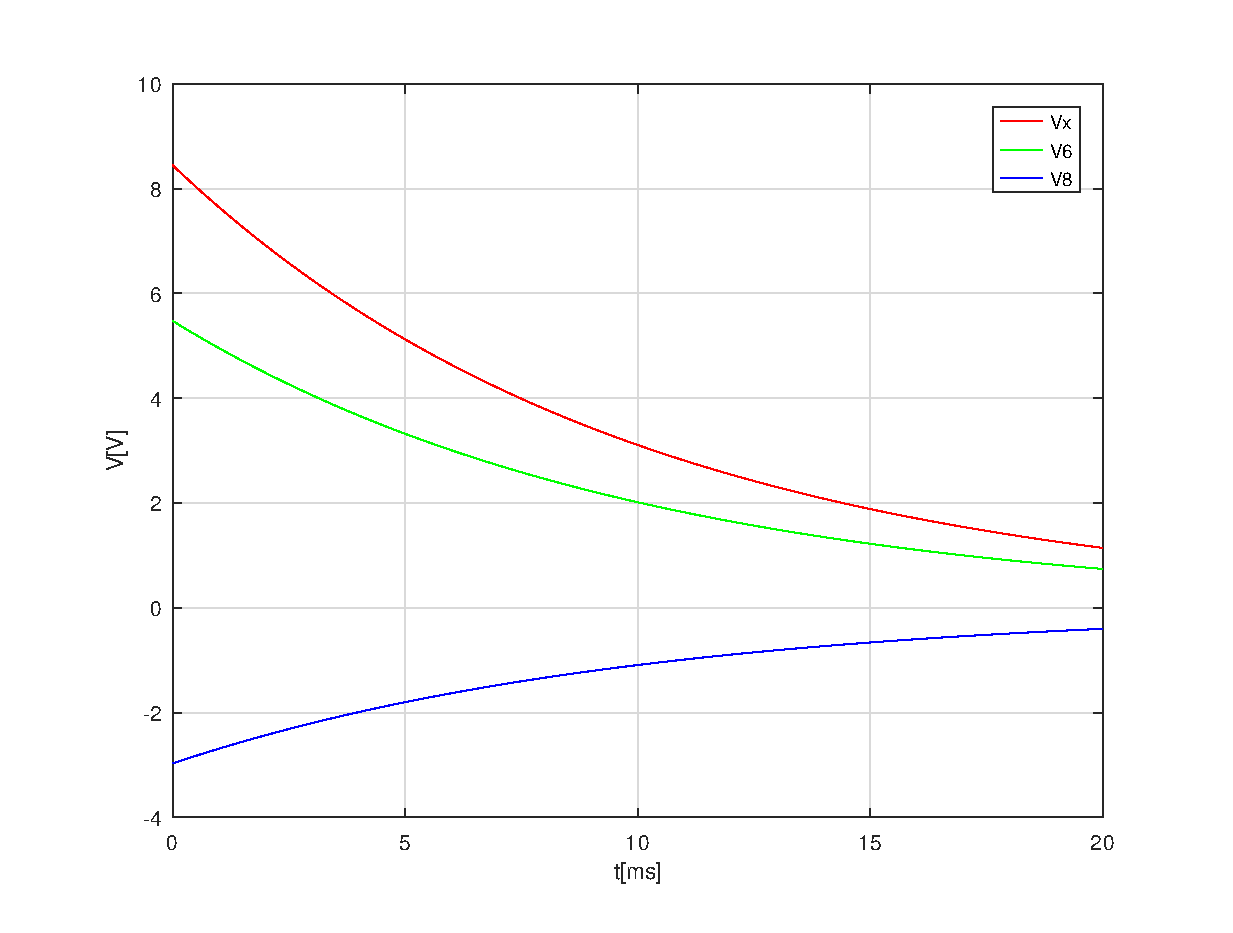
\includegraphics[width=.95\linewidth]{Natural.eps}
  \caption{Octave}
\end{subfigure}%
\begin{subfigure}{.5\textwidth}
  \centering
  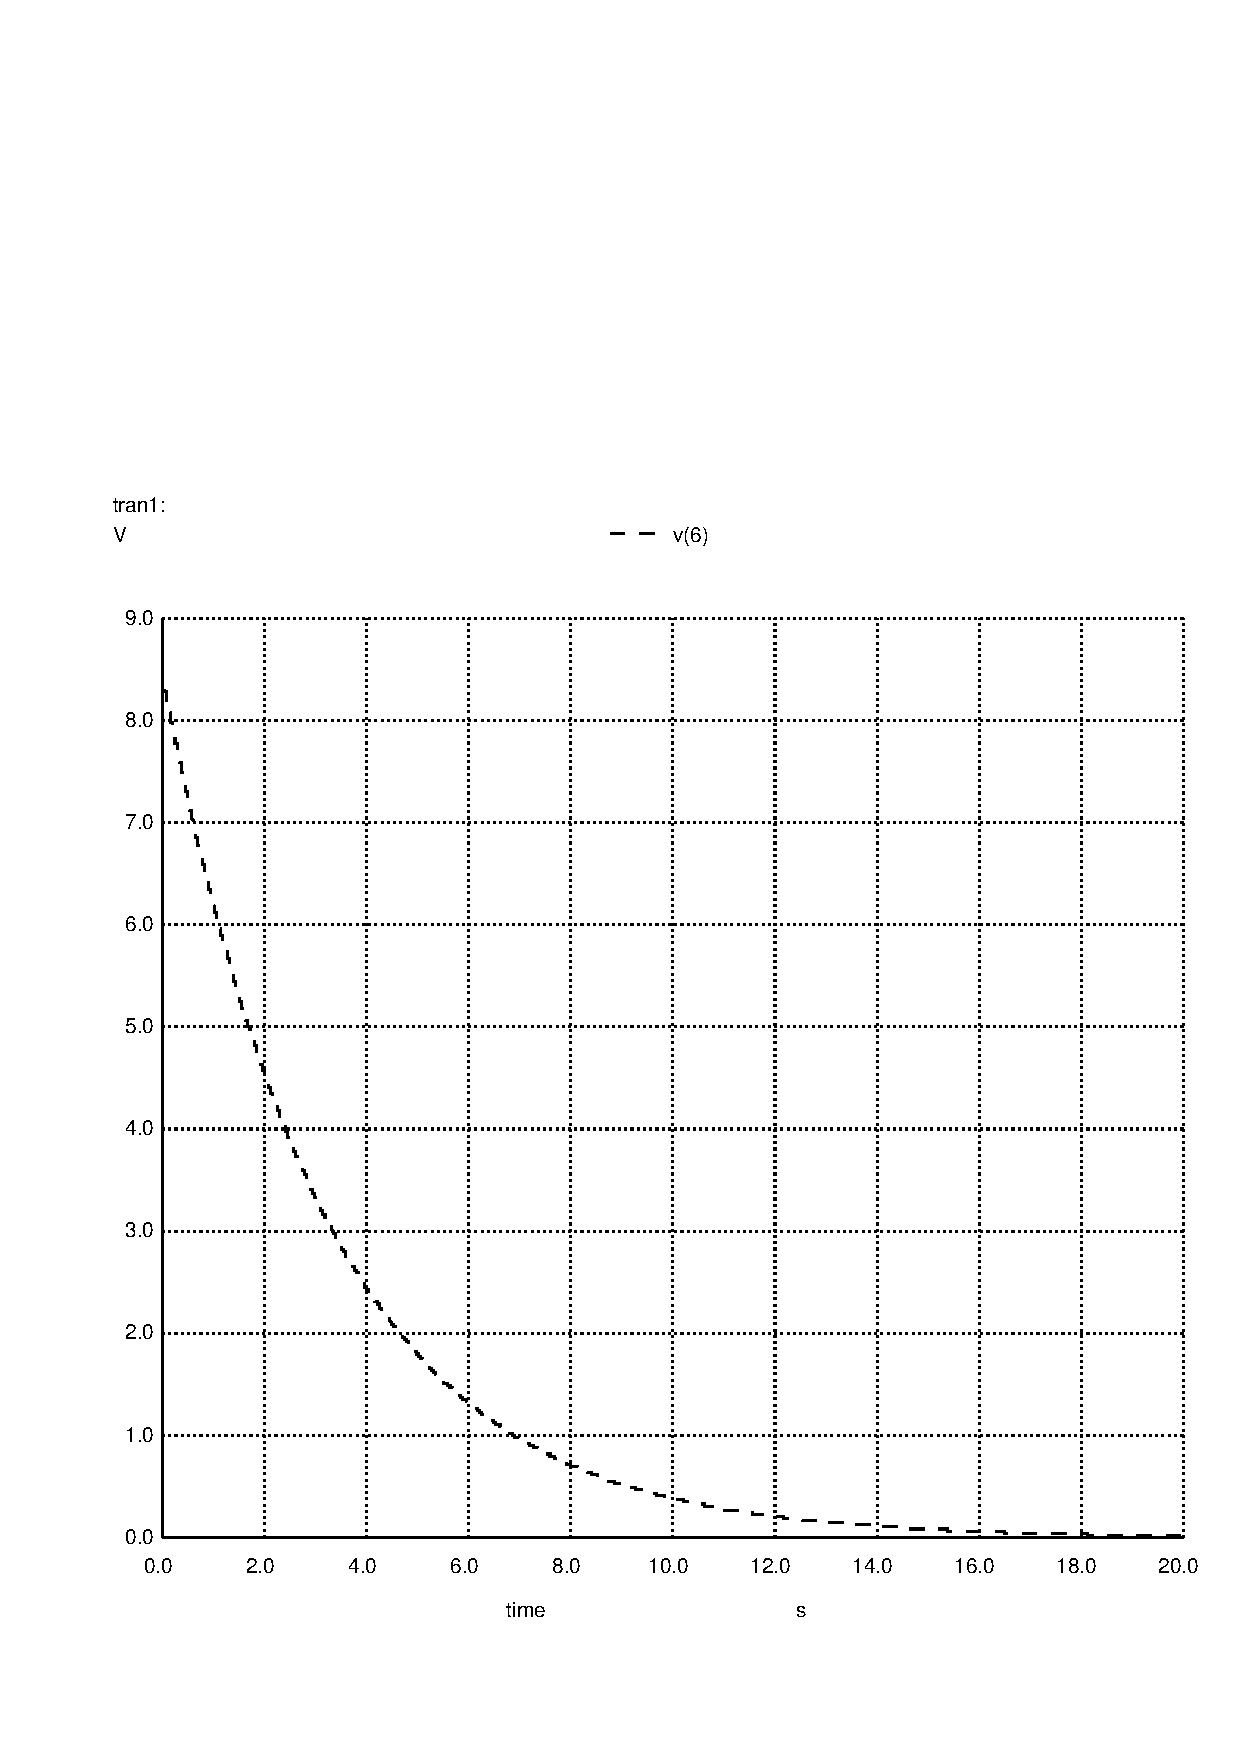
\includegraphics[width=.75\linewidth, trim={2cm 1.5cm 0.5cm 6cm}, clip]{../Simulation/trans_nat.pdf}
  \caption{Ngspice}
\end{subfigure}
\caption{Natural response}
\label{fig:test}
\end{figure}


\indent

As expected the voltages decrease exponentially with time, this represents the capacitor being discharged. Furthermore, it can be seen that the voltage on $V_8$ is zero and that the lines of $V_6$ and $V_x$ are overlapping, meaning the relation $V_x = V_6$ is proved.

\subsubsection{Transient analysis: Final solution}

\indent


\begin{figure}[H]
\centering
\begin{subfigure}{.5\textwidth}
  \centering
  \includegraphics[width=.95\linewidth]{FinalResponse.eps}
  \caption{Octave}
\end{subfigure}%
\begin{subfigure}{.5\textwidth}
  \centering
  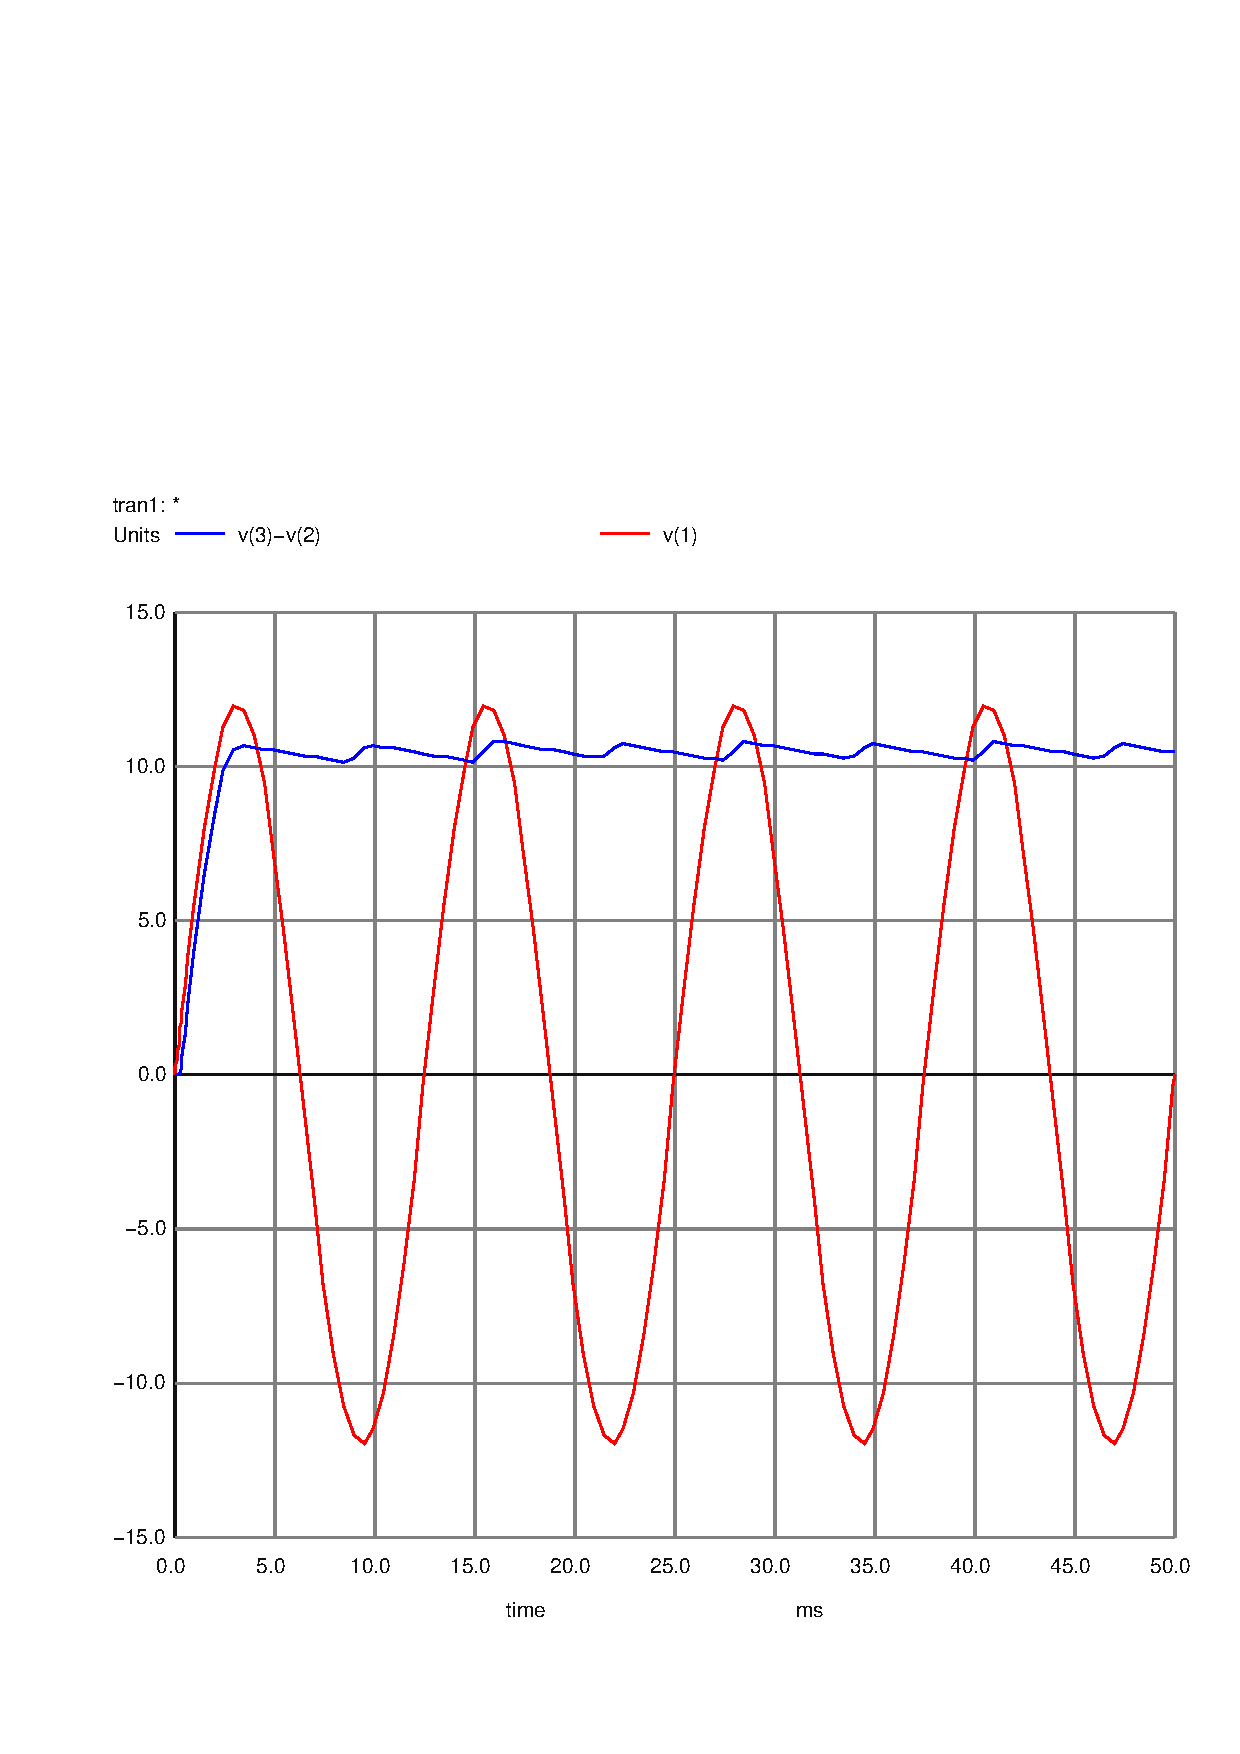
\includegraphics[width=.75\linewidth, trim={2cm 1.5cm 0.5cm 6cm}, clip]{../Simulation/trans_forc.pdf}
  \caption{Ngspice}
\end{subfigure}
\caption{Natural response}
\label{fig:test}
\end{figure}



One aspect that should be mentioned about this data is that the phase of the capacitor is offset to the voltage source by approximately $180^\circ$, and $V_c$ is offset by approximately $90^\circ$. Therefore, its possible to deduce that the current's frequency is greater than the cut-off frequency of this low pass filter (this topic will be further analysed below, on section \ref{sec:Frequency analysis}).
Moreover, $V_x$ decreases with time, approaching zero, but maintains the oscillating regime. This means the capacitor is being discharged until its average is zero. Once this happens the capacitor is lightly charged and discharged in the same frequency as the source.

\subsubsection{Frequency analysis}
\label{sec:Frequency analysis}

\indent



\begin{figure}[H]
\centering
\begin{subfigure}{.5\textwidth}
  \centering
  \includegraphics[width=.95\linewidth]{Magnitude.eps}
  \caption{Octave}
\end{subfigure}%
\begin{subfigure}{.5\textwidth}
  \centering
  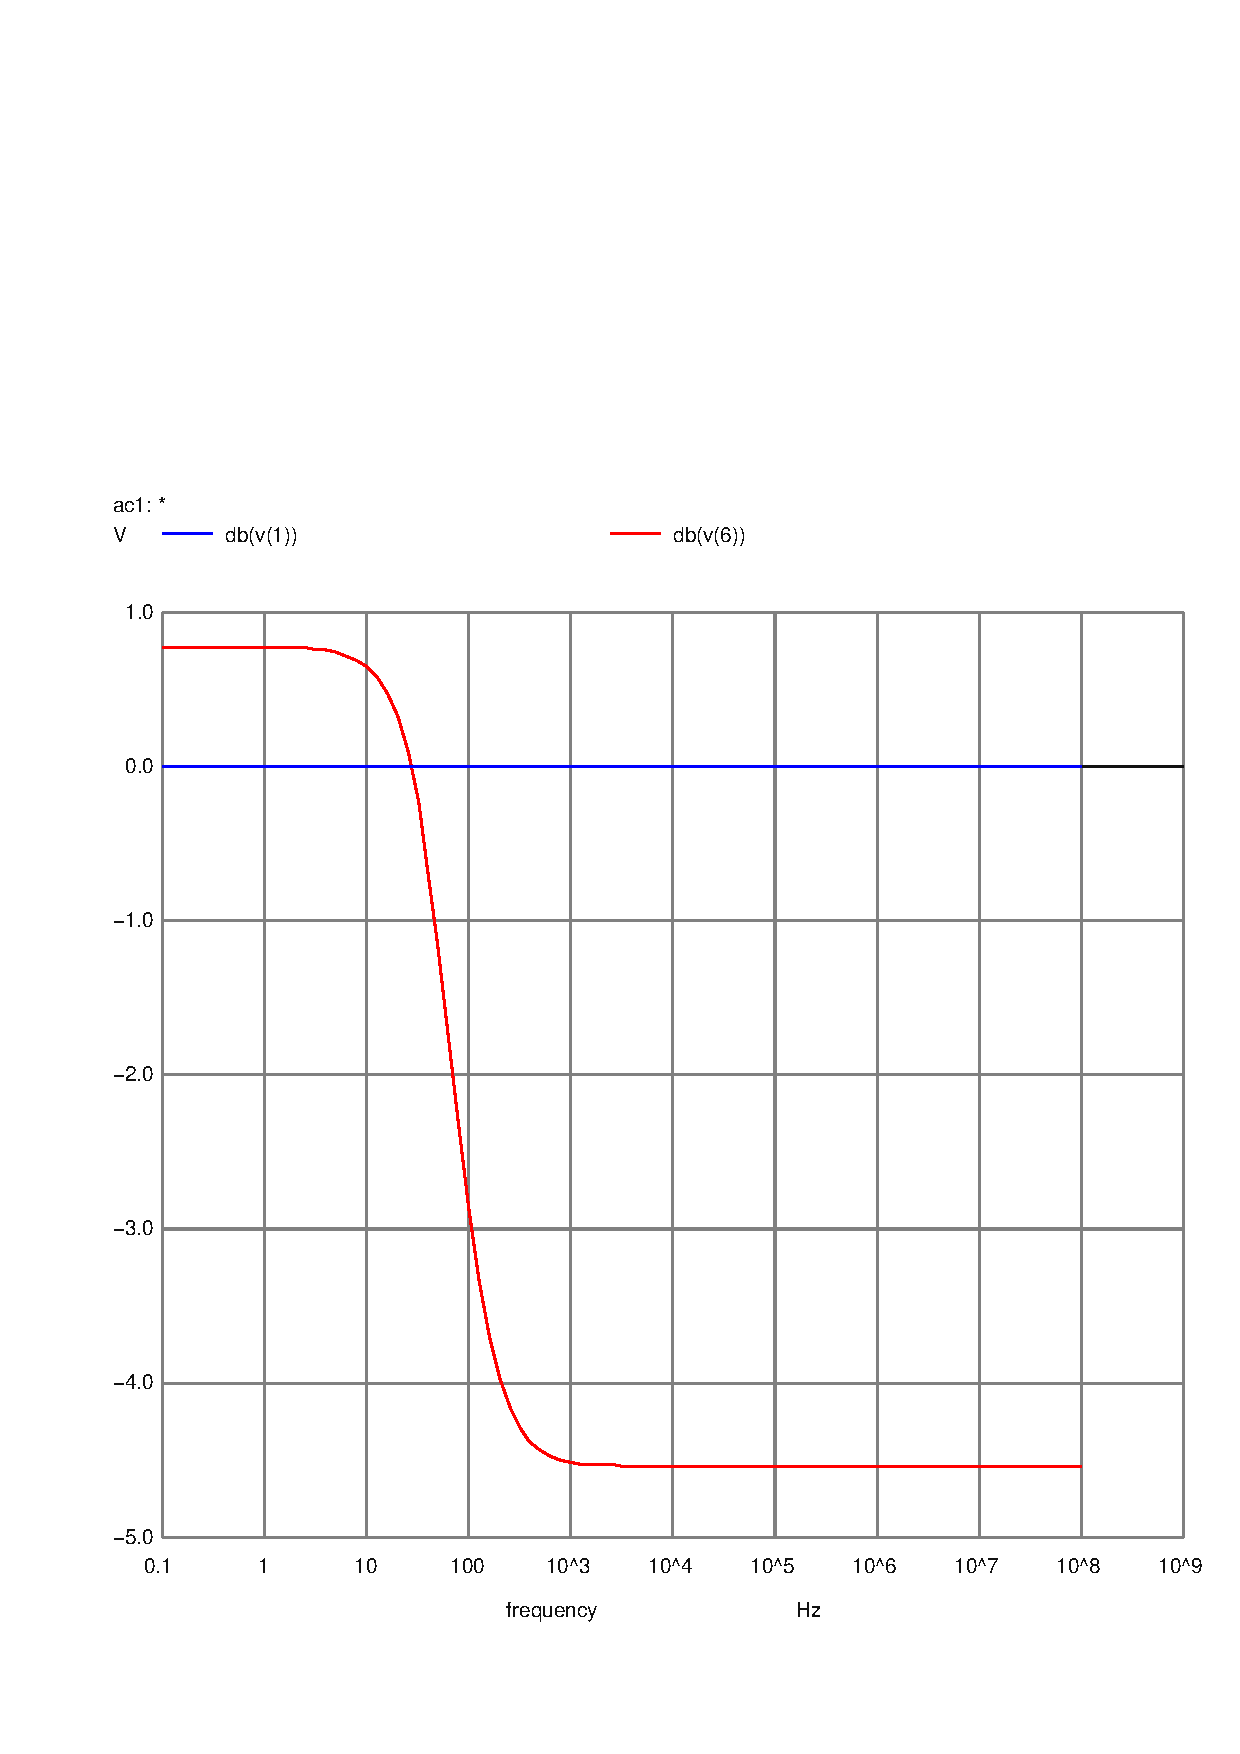
\includegraphics[width=.75\linewidth, trim={2cm 1.5cm 0.5cm 6cm}, clip]{../Simulation/acm_db.pdf}
  \caption{Ngspice}
\end{subfigure}
\caption{Natural response}
\label{fig:test}
\end{figure}



\begin{figure}[H]
\centering
\begin{subfigure}{.5\textwidth}
  \centering
  \includegraphics[width=.95\linewidth]{Phase.eps}
  \caption{Octave}
\end{subfigure}%
\begin{subfigure}{.5\textwidth}
  \centering
  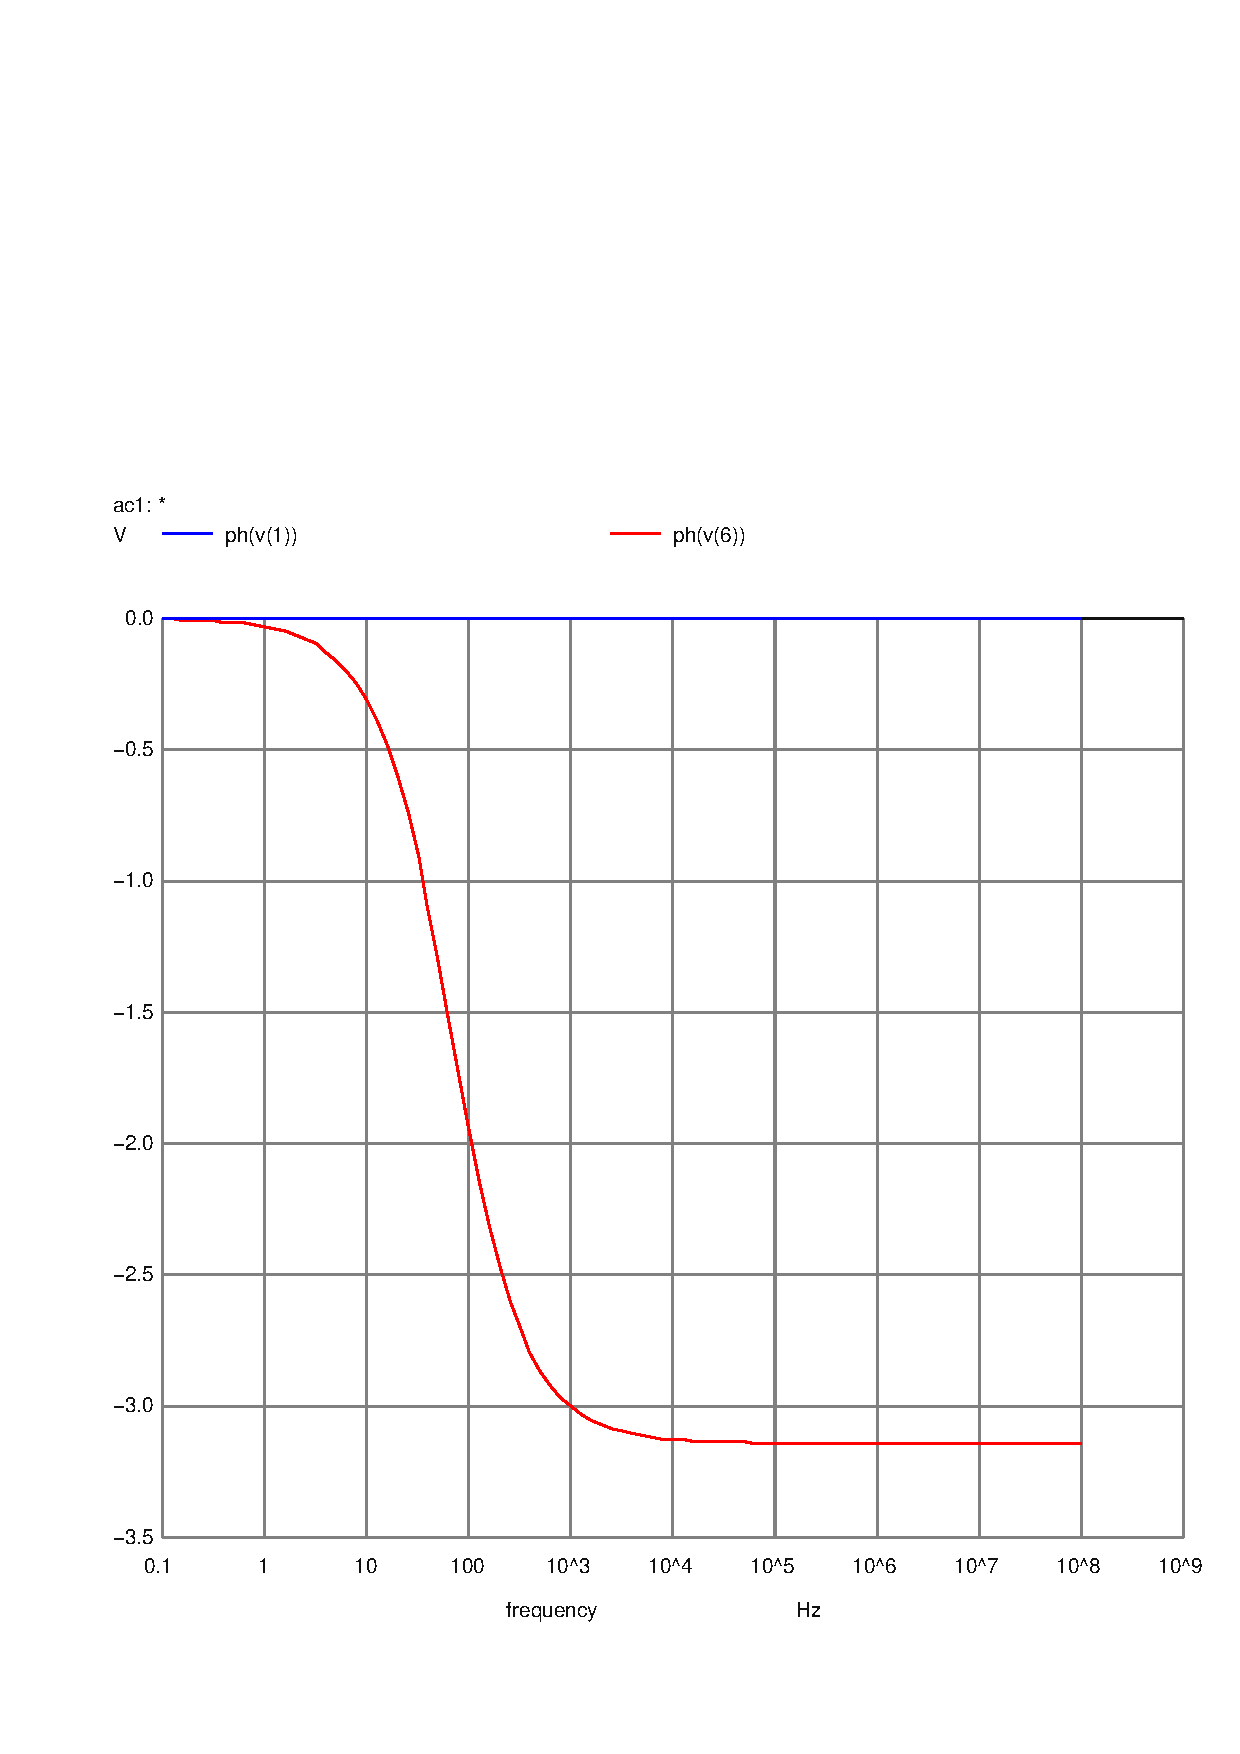
\includegraphics[width=.75\linewidth, trim={2cm 1.5cm 0.5cm 6cm}, clip]{../Simulation/acph.pdf}
  \caption{Ngspice}
\end{subfigure}
\caption{Natural response}
\label{fig:test}
\end{figure}



$V_s$ remains constant since it is the voltage that was taken as the reference (it is an independent voltage source). $V_6$ and $V_c$, on the other hand, have an asymptotic behaviour, tending to offset $-180^\circ$ and $-90^\circ$, respectively.

These graphs confirm that the circuit can be classified as a low-pass filter, since, for low frequencies, the magnitude of voltage on the capacitor ($V_6-V_8$) is close to the one from the voltage source. However this changes on high frequencies, the voltage drops drastically if the frequency increases.

As seen on figure \ref{fig:FreqPhOc}, the cutoff frequency is around $50 Hz$. This value can be confirmed by calculating it according to the equation \ref{eq:cutoff}: \input{../Analysis/Cutoff.tex} Hz. By definition, this frequency is the one with a phase of $45^\circ$.

\begin{equation}
    f_{cutoff} = \frac{1}{2\pi \cdot R_{eq} \cdot C} \hspace{5pt}.
    \label{eq:cutoff}
\end{equation}

\section{Conclusion}
\label{sec:conclusion}

\indent

In this laboratory assignment, the objective of analysing a circuit with a capacitor has been achieved. This circuit has been analysed using \textit{Operating point}, \textit{transient} and \textit{frequency} analysis. The \textit{Operating point} analysis was conducted like in the previous laboratory assignment, using node and mesh analysis. The \textit{transient} and \textit{frequency} analysis were based on phasors and on the nodal method using imaginary numbers.


The theoretical section has been solved using the {\em Octave} Maths tool to compute all the previous values. Those results were then confronted with the simulation results, which were obtained by using the {\em Ngspice} tool, resulting in an almost perfect match (with a level of precision of $10^{-5}$).

%\cleardoublepage

% ----------------------------------------------------------------------
%  Bibliography
% ----------------------------------------------------------------------
%\addcontentsline{toc}{section}{\bibname}
%\bibliographystyle{abbrvunsrtnat} % <<<<< SELECT IF USING REFERENCES BY NUMBER (CITATION ORDER)
%\bibliography{../../../BIBfile.bib}

% ----------------------------------------------------------------------
\end{document}
% ----------------------------------------------------------------------

